\section{Methods}
\label{methods}
%From ILO:
%"Plan and carry out a small-scale investigation of an algorithmic research problem. This investigation could be theoretical, experimental, or both."
This section will cover the methods used throughout the project and attempt to reason about these. The motivation behind each method is to support the problem definition and the analysis of the \qs{} implementation. The analysis consists of verifying the correctness of the stated results and applying the implementation with other data inputs to verify the relation between \qs{} and the baseline. Furthermore a number of practical tests are conducted to research possible performance gains.

\subsection{Experiment verification}

\subsubsection{Baseline comparison}
The paper compares the \qs{} performance with other compression algorithms, including (\pq{}) and a simple baseline algorithm, \gr{}. In order to verify their results, a version of Grid has been implemented as baseline to use for replication experiments. The basic concept is to make a range of buckets over each dimension for the point set. Each point will have its value for a dimension reduced to the value of the bucket in which the points value lies. By doing so, the value of the point can be stored with fewer bits and thus compress the data set.

\subsubsection{Other datasets}
To ensure proper verification of the results for the \qs{}, the implementation and baseline is tested on another dataset not included in the paper. If the results from another dataset somewhat match the results given in the paper \cite{wagner17}, it will strengthen the credibility of the practical efficiency of the \qs{} implementation.
\\
\\
The choice of other datasets could provide some additional insight into how the properties of some dataset might impact the optimality of the parameters given to the \qs{}. It might be interesting to feed datasets with different properties to the \qs{}, as results may change from very sparse / spread out datasets to very dense datasets.

\subsection{Experimenting with possible improvements}
A number of experiments have been conducted in an attempt to improve \qs{}. The approaches and experiments will be elaborated below.
%EMil vil gerne have "on" med

\subsubsection{Random bits}
This expirement focuses on the pruning step of the algorithm. Recall that in the pruning step \qs{} shifts each point in a quad towards the lower left corner by replacing existing bits with zero's. The alteration introduced in this expiriment moves each point in a qaud towards a random corner of that quad. More precisely, by not only introducing zero's into the bit string as replacement, this feature random valued bits into the bit string. This might improve the resulting sketch by pulling the point in an arbitraryt direction for each dimension rather than only distorting them in one direction.  This could potentially improve some scenarios of the sketch where the points are either . A visualization of this can be seen on figure \ref{fig:randombits}, where the transformation by \qs{} is referred to as QS, and the transformation by \qsr{} is referred to as QSR. In the graphical representation each point lies next to eachother if they are placed in the same corner, where in the actual transformation these will have the exact same coordinates. 
\begin{figure}[h]
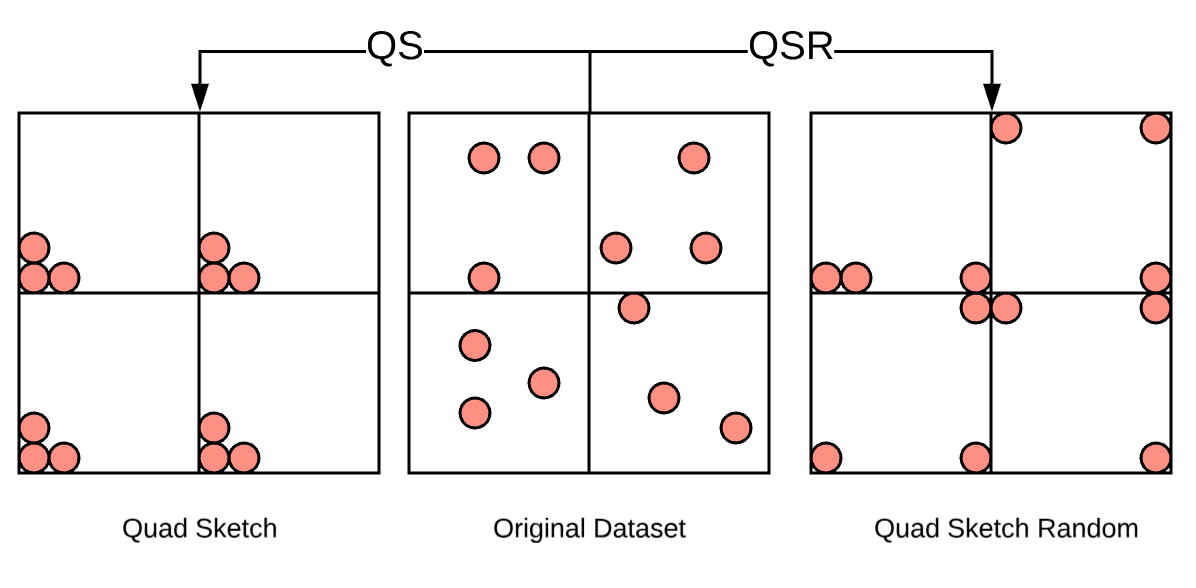
\includegraphics[width=1\textwidth]{figures/randombits}
\caption{Random Bit Demonstration}
\label{fig:randombits}
\end{figure}
The given example in figure \ref{fig:randombits} demonstrates a scenario where the expirement performs decently. It should be noted that the random movement of the points could also result in a worse representation. Such a scenario is described in \ref{disc/threats/randomness}.
\\
\\
The motivation of this expirement stems from the creation of the random quad tree in \qs{}. Should the creation of this quadtree accidentaly quad through closely clustered points then the distortion could be quite severe. By introducing randomness into the direction of the points, they might end up in corners closer to each other and thereby reduce the amount of distortion.  
\clearpage